\documentclass[11pt]{article}

\usepackage[a4paper, margin=1in]{geometry}
\usepackage{amsmath, amssymb, amsthm}
\usepackage{mathtools}
\usepackage{algorithm}
\usepackage{algpseudocode}
\usepackage{booktabs}
\usepackage{enumitem}
\usepackage{hyperref}
\usepackage{tikz}
\usepackage{pgfplots}
\pgfplotsset{compat=1.18}
\usetikzlibrary{positioning, arrows.meta, shapes.geometric}

\hypersetup{
    colorlinks=true,
    linkcolor=blue!70!black,
    citecolor=blue!70!black,
    urlcolor=blue!70!black
}

% ── Theorem environments ──────────────────────────────────────────────────────
\newtheorem{theorem}{Theorem}[section]
\newtheorem{proposition}[theorem]{Proposition}
\newtheorem{lemma}[theorem]{Lemma}
\newtheorem{corollary}[theorem]{Corollary}
\newtheorem{definition}[theorem]{Definition}
\newtheorem{remark}[theorem]{Remark}
\newtheorem{example}[theorem]{Example}

% ── Math macros ───────────────────────────────────────────────────────────────
\newcommand{\dist}{\operatorname{dist}}
\newcommand{\UDG}{\operatorname{UDG}}
\newcommand{\Efalse}{E_{\mathrm{false}}}
\newcommand{\Etrue}{E_{\mathrm{true}}}
\newcommand{\chihat}{\widehat{\chi}}
\newcommand{\R}{\mathbb{R}}

% ─────────────────────────────────────────────────────────────────────────────
\title{%
  \textbf{Safe Near-UDG Transformations for Graph Coloring}\\[0.4em]
  \large A Polynomial-Time Compiler for Neutral-Atom Quantum Hardware
}
\author{}
\date{\today}

\begin{document}
\maketitle
\tableofcontents
\newpage

% =============================================================================
\section{Overview and Motivation}
% =============================================================================

Let $G = (V, E)$ be an arbitrary input graph with chromatic number $\chi(G)$.
The goal is to find a \emph{Unit Disk Graph} (UDG) $H = (V, E_H)$ together
with a placement $p : V \to \R^2$ and a radius $r > 0$ such that:
\begin{enumerate}
  \item $H = \UDG(p, r)$, i.e., $(u,v) \in E_H \iff \|p(u)-p(v)\|_2 \leq r$.
  \item $E(G) \subseteq E(H)$ \quad (\emph{safety invariant}).
  \item $\chi(H) \approx \chi(G)$ \quad (\emph{low coloring inflation}).
\end{enumerate}

The safety invariant ensures that every proper coloring of $H$ is
automatically a proper coloring of $G$, giving a \textbf{trivially correct
decoder}: restrict the coloring of $H$ to the original vertex set.

\subsection{Why This Approach Avoids NP-Completeness}

Exact UDG embedding (deciding whether $G$ itself is a UDG) is NP-hard \cite{Breu1998,Jungck2021}.
However, we do \emph{not} ask whether $G$ is a UDG. We ask for a UDG
\emph{supergraph} $H \supseteq G$, which can always be trivially constructed
(e.g., place all atoms at a single point and set $r = 1$). The research
question is therefore: \emph{how good} can we make $H$ in polynomial time?
Every heuristic below runs in polynomial time per step \cite{Cormen2009}, and the cumulative
pipeline has complexity $O(T|V|^2)$ dominated by the optimization loop.

\subsection{Key Definitions}

\begin{definition}[False Edges]
Given a safe UDG supergraph $H$ of $G$, the \emph{false edges} are
\[
  \Efalse = E(H) \setminus E(G).
\]
These are edges present in $H$ but absent in $G$.
\end{definition}

\begin{definition}[Color Inflation]
The \emph{color inflation ratio} is
\[
  \rho = \frac{\chihat(H)}{\chihat(G)},
\]
where $\chihat$ denotes a heuristic estimate of the chromatic number
(e.g., from DSATUR).  The goal is $\rho \approx 1$.
\end{definition}

\begin{proposition}[Safety $\Rightarrow$ Decoder Correctness]
\label{prop:safety}
If $E(G) \subseteq E(H)$ and $\kappa_H : V \to \{1,\dots,k\}$ is a proper
coloring of $H$, then $\kappa_H$ is also a proper coloring of $G$.
\end{proposition}

\begin{proof}
For every edge $(u,v) \in E(G)$, we have $(u,v) \in E(H)$, so
$\kappa_H(u) \neq \kappa_H(v)$.  Hence $\kappa_H$ satisfies all constraints
of $G$.
\end{proof}

This proposition is the \textbf{main correctness guarantee} of the entire
framework and holds for any supergraph, regardless of which heuristic is used
to construct $H$.

\newpage

% =============================================================================
\section{Heuristic 1 — Geometric Loss Minimization}
% =============================================================================

\subsection{Description}

Place vertices via a differentiable coordinate map $p : V \to \R^2$ and
optimize the loss using gradient-based methods \cite{Nesterov2004, Boyd2004}:
\[
  L_{\mathrm{geom}}(p, r)
  =
  \underbrace{\sum_{(u,v)\in E(G)} \max(0,\, d_{uv} - r)^2}_{\text{pull true
  edges inside radius}}
  +\;
  \lambda
  \underbrace{\sum_{(u,v)\notin E(G)} \max(0,\, r + \epsilon -
  d_{uv})^2}_{\text{push non-edges outside radius}}
  +\;
  \mu \cdot r^2.
\]
Here $d_{uv} = \|p(u) - p(v)\|_2$, and the terms work as follows:
\begin{itemize}
  \item \textbf{Term 1:} Penalizes true edges whose distance exceeds $r$.  Ensures edges are pulled inside the interaction radius.
  \item \textbf{Term 2:} Penalizes non-edges whose distance falls below $r + \epsilon$. Pushes non-edges outside with a safety margin $\epsilon > 0$.
  \item \textbf{Term 3:} Regularization preventing $r \to \infty$.  With weight $\mu > 0$, this avoids the trivial solution (complete graph).
\end{itemize}

\subsection{Critical Refinement: Joint Optimization of $r$}

The original formulation had a circular dependency: $r$ was fixed during
optimization and recomputed afterward. This can lead to safety violations after
the final gradient step.

\textbf{Refined approach:} Treat $r$ as a \textbf{joint optimization variable}.
Compute gradients with respect to both $p$ and $r$:
\[
  p \leftarrow p - \eta \nabla_p L, \quad r \leftarrow r - \eta \nabla_r L.
\]
After optimization terminates, perform a \textbf{hard safety check}:
\[
  E(G) \subseteq E_H \stackrel{?}{\subseteq} \{(u,v) : d_{uv} \leq r\}.
\]
If the check fails, set $r \leftarrow \max_{(u,v)\in E(G)} d_{uv} + \delta$ for
a small $\delta > 0$ and rebuild $H$.

\subsection{Complexity}

Each gradient step costs $O(|V|^2 + |E|)$ (the non-edge sum dominates when
the graph is dense). Total cost: $O\!\left(T(|V|^2 + |E|)\right)$ for $T$
iterations. This is polynomial for any fixed $T$.

\subsection{Example: Path Graph $P_4$}

\begin{example}
Graph: $v_1 - v_2 - v_3 - v_4$ (4 vertices, 3 edges in a line).

\medskip\noindent
\textbf{Bad initial placement:} Spread vertices along a long line.
\begin{align*}
  p(v_1) &= (0, 0), & p(v_2) &= (100, 0),\\
  p(v_3) &= (200, 0), & p(v_4) &= (300, 0).
\end{align*}
All edge distances are 100, non-edge distances are 200 or 300. To include all
edges, radius $r = 100$ is needed.

\medskip\noindent
\textbf{Good placement after optimization:} Compress vertices tightly.
\begin{align*}
  p(v_1) &= (0, 0), & p(v_2) &= (0.6, 0),\\
  p(v_3) &= (1.2, 0), & p(v_4) &= (1.8, 0).
\end{align*}
All edge distances are 0.6, non-edge distances are 1.2 or 1.8. Radius $r = 0.6$
suffices. Much tighter — better for hardware.
\end{example}

\newpage

% =============================================================================
\section{Heuristic 2 — Color-Danger Weighted Penalty}
% =============================================================================

\subsection{Description}

Compute a heuristic coloring $\kappa_G : V \to \{1,\dots,k\}$ of $G$ first
(using DSATUR algorithm for better quality 	te{Brelaz1979}). Assign weights:
\[
  w_{uv} =
  \begin{cases}
    M, & \kappa_G(u) = \kappa_G(v) \quad \text{(same color — dangerous)},\\
    1, & \text{otherwise},
  \end{cases}
\]
with $M \gg 1$ (typically $M = 100$). Use the weighted loss:
\[
  L_{\mathrm{color}}(p,r)
  =
  \sum_{(u,v)\in E(G)} \max(0,\, d_{uv} - r)^2
  +
  \lambda \sum_{(u,v)\notin E(G)}
  w_{uv}\max(0,\, r + \epsilon - d_{uv})^2.
\]

\subsection{Key Theorem: Color-Safe Embedding}

\begin{theorem}[Color-Safe Embedding]
\label{thm:colorsafe}
Suppose the optimization produces a placement such that all same-color non-adjacent
pairs satisfy $d_{uv} > r$. Then $\kappa_G$ is a valid proper coloring of $H$, and
\[
  \chi(H) \leq k.
\]
Combined with $\chi(G) \leq \chi(H)$, we have $\chi(G) \leq \chi(H) \leq k$.
If $k \approx \chi(G)$, then $\rho \approx 1$.
\end{theorem}

\begin{proof}
By assumption, for every non-edge $(u,v) \notin E(G)$ with $\kappa_G(u) =
\kappa_G(v)$, we have $d_{uv} > r$, so $(u,v) \notin E(H)$.  Each color
class of $\kappa_G$ is therefore an independent set in $H$.  A $k$-coloring
of $H$ using $\kappa_G$ is proper.
\end{proof}

\subsection{Refinement: Use DSATUR for Initial Coloring}

The quality of the heuristic depends on the quality of $\kappa_G$.  Greedy coloring
can use up to $\chi(G) + \Delta$ colors (where $\Delta$ is max degree),
which may overestimate.

\textbf{Refined approach:} Use the \textbf{DSATUR} (Brelaz's algorithm) \cite{Brelaz1979}
instead of greedy coloring. DSATUR runs in $O(|V|^2)$ and produces
significantly better colorings on average, especially for structured graphs.
For sparse graphs, a largest-first vertex ordering with greedy coloring \cite{Welsh1967}
is a reasonable alternative in $O(|V| + |E|)$.

\subsection{Example: Path Graph $P_3$}

\begin{example}
Graph: $v_1 - v_2 - v_3$ (path on 3 vertices).  True edges: $(v_1,v_2), (v_2,v_3)$.
Non-edge: $(v_1,v_3)$.

DSATUR coloring: $\kappa_G(v_1) = 1, \kappa_G(v_2) = 2, \kappa_G(v_3) = 1$.
Same-color pair: $(v_1, v_3)$ with $\kappa_G(v_1) = \kappa_G(v_3) = 1$ (dangerous).

Without weighting (Heuristic 1 alone): False edge $(v_1, v_3)$ gets penalty 1.0.

With weighting (Heuristic 2): Same-color pair $(v_1, v_3)$ gets penalty $M \times 1.0 = 100.0$
(much larger). The optimizer strongly penalizes this configuration and pushes
$v_1$ and $v_3$ far apart. Result: the original 2-coloring is preserved with
zero inflation.
\end{example}

\newpage

% =============================================================================
\section{Heuristic 3 — Clique Inflation Control}
% =============================================================================

\subsection{Description}

Since $\omega(H) \leq \chi(H)$ (clique number lower-bounds chromatic number),
accidental large cliques in $H$ form a lower bound on coloring inflation.
The heuristic detects dense neighborhoods in $H$ and pushes the corresponding
vertices apart.

\subsection{Hardware-Specific Observation: Bounded Cliques in Neutral Atoms}

\begin{proposition}[Hardware-Bounded Cliques]
In a physical neutral-atom UDG with interaction radius $r$ and minimum atom
spacing $d_{\min}$ (a hardware constant, typically $2$--$4\,\mu\mathrm{m}$),
the maximum clique size is bounded by:
\[
  \omega_{\max} \leq \left\lfloor \frac{\pi r^2}{c \cdot d_{\min}^2}
  \right\rfloor,
\]
where $c$ is a packing constant (approximately $0.9$ for close packing in 2D) \cite{Heppes2003}.
\end{proposition}

This hardware-derived bound is unique to the neutral-atom setting \cite{Henriet2021, Scholl2022}
and provides an a priori upper bound on $\chi(H)$ that depends on physical parameters. This
should be prominently featured in the thesis as a key contribution linking
hardware constraints to algorithmic design.

\subsection{Practical Clique Detection}

General clique detection is NP-hard \cite{Bomze1999}. However, in a UDG, every clique is
geometrically local: all vertices within a clique lie within a disk of radius
$r$. Therefore, every clique is contained within the closed neighborhood $N[v]$
of some vertex $v$.

Detection within local neighborhoods costs $O(\Delta^2)$ per vertex (where
$\Delta$ is max degree), giving $O(|V|\Delta^2)$ overall. For hardware-feasible
atom counts ($|V| \lesssim 10^3$), this is practical.

\subsection{Termination Guarantee via Monotone Potential}

Define the weighted false-edge cost:
\[
  \Phi = \sum_{(u,v) \in \Efalse} w_{uv},
\]
using the same weights $w_{uv}$ as Heuristic 2. Accept a repair step only if
$\Phi$ strictly decreases. This ensures termination in finitely many steps
with bounded step size.

\subsection{Example: Accidental 5-Clique in $K_4$}

\begin{example}
Original graph: $K_4$ ($\chi(K_4) = 4$).

Bad placement: All four vertices clustered tightly:
$p(v_1) = (0, 0), p(v_2) = (0.1, 0), p(v_3) = (0, 0.1), p(v_4) = (0.1, 0.1)$.
Max distance: $\approx 0.14$. Set $r = 0.2$.

Spurious vertex $v_5$ (not in original graph) placed at $(0.05, 0.05)$.
Distance from $v_5$ to all others: $\approx 0.07 < 0.2$. Now $\{v_1, v_2, v_3,
v_4, v_5\}$ forms a 5-clique in $H$, forcing $\chi(H) \geq 5 > \chi(G) = 4$.

Clique repair detects this and pushes $v_5$ outward to $(2, 2)$, placing it
outside the radius. The 5-clique breaks, and $\chi(H)$ returns to 4.
\end{example}

\newpage

% =============================================================================
\section{Heuristic 4 — Laplacian Eigenmap Initialization}
% =============================================================================

\subsection{Clarification: Initialization, Not Standalone Heuristic}

Heuristic 4 is an \textbf{initialization strategy} for Heuristics 1 and 2, not
a standalone optimization step. The thesis should be explicit about this
distinction: a good initialization determines the basin of attraction for
subsequent gradient descent and substantially impacts convergence speed and
quality.

\subsection{The Laplacian Eigenmap Method}

The graph Laplacian is defined as $L = D - A$ \cite{Chung1997}, where $D$ is the degree matrix
and $A$ is the adjacency matrix. The eigenvectors of $L$ provide a natural
low-dimensional embedding of the graph.

For 2D placement, use the second and third smallest eigenvectors $\phi_2$ and
$\phi_3$ (the Fiedler vector \cite{Fiedler1973} and the next):
\[
  p_0(v_i) = (\phi_2(i), \phi_3(i)).
\]

\subsection{Why It Works for Coloring}

The Laplacian eigenmap \cite{Belkin2003} has the following properties:
\begin{itemize}
  \item \textbf{Adjacent vertices are placed near:} The quadratic form
    $\phi^\top L \phi$ is minimized when neighbors are close, so the eigenvectors
    naturally place adjacent vertices nearby.
  \item \textbf{Non-adjacent vertices are placed far:} Vertices in different
    parts of the graph (especially those in different color classes) are
    assigned opposite signs or distant values by the spectral structure.
  \item \textbf{Color classes are separated:} Since vertices in the same color
    class are non-adjacent, they tend to be placed far apart, reducing
    same-color false edges before optimization begins.
\end{itemize}

This initialization is particularly effective for bipartite graphs, trees, and
sparse graphs where the spectral structure strongly reflects the coloring
structure.

\subsection{Complexity}

Eigendecomposition costs $O(|V|^2)$ using dense methods or $O(|V| \cdot k)$ using
sparse solvers (where $k$ is the number of eigenvectors computed, typically
$k = 3$). This is a one-time cost, not amortized over the iteration count.

\subsection{Example: Bipartite Graph $K_{2,2}$}

\begin{example}
Graph: Two parts $A = \{u_1, u_2\}$ and $B = \{v_1, v_2\}$, with all cross
edges and no edges within parts. This is $K_{2,2}$, bipartite with $\chi = 2$.

The Fiedler vector naturally assigns positive values to $A$ and negative values
to $B$ (or vice versa):
\[
  \phi_2 \approx (1, 1, -1, -1)^T / 2.
\]
The eigenmap places all $A$-vertices on one side of the 2D layout and all
$B$-vertices on the opposite side:
\begin{align*}
  p_0(u_1) &\approx (0.5, y_1), & p_0(u_2) &\approx (0.5, y_2),\\
  p_0(v_1) &\approx (-0.5, y_3), & p_0(v_2) &\approx (-0.5, y_4).
\end{align*}
Same-color pairs (e.g., $(u_1, u_2)$) are already far apart. The optimizer
needs minimal adjustment. This is exactly the geometry needed for chromatic
preservation.
\end{example}

\newpage

% =============================================================================
\section{Heuristic 5 — Local False-Edge Repair}
% =============================================================================

\subsection{Description}

After global optimization, identify harmful false edges and adjust coordinates
locally. For each harmful false edge $(u,v)$, push the vertices apart:
\begin{align*}
  p(u) &\leftarrow p(u) + \eta\,\frac{p(u) - p(v)}{\|p(u) - p(v)\|},\\
  p(v) &\leftarrow p(v) + \eta\,\frac{p(v) - p(u)}{\|p(v) - p(u)\|}.
\end{align*}
After each push step, repair any true edge $(a,b) \in E(G)$ whose distance exceeded
$r$ by applying a symmetric pull step with negative step size.

\subsection{Harmfulness Criteria}

A false edge $(u,v) \in \Efalse$ is \emph{harmful} if:
\begin{enumerate}
  \item it connects vertices with the same color in $\kappa_G$ (cheapest check, $O(1)$),
  \item it participates in a large clique of $H$,
  \item it would increase $\chihat(H)$ if tested,
  \item it breaks a large independent set of $G$.
\end{enumerate}
Criterion 1 should gate the others for efficiency.

\subsection{Termination Guarantee via Monotone Potential}

Without a termination guarantee, the repair loop can oscillate. The refinement
uses the same weighted false-edge cost:
\[
  \Phi = \sum_{(u,v) \in \Efalse} w_{uv},
\]
where $w_{uv} = 100$ if same color, $1$ otherwise. Accept a repair step only
if $\Phi$ strictly decreases. With bounded step size and finite precision,
this terminates in finitely many steps. Set a maximum iteration count as a
hard fallback.

\subsection{Complexity}

Each repair iteration costs $O(|\Efalse| \cdot |V|)$ (identifying harmful edges
and coordinate updates). Total: $O(T \cdot |\Efalse| \cdot |V|)$ for $T$
iterations.

\subsection{Example: Path $P_4$ with Local False Edge}

\begin{example}
Graph: $v_1 - v_2 - v_3 - v_4$. Coloring: $\kappa_G = (1, 2, 1, 2)$.

Placement after global optimization:
\begin{align*}
  p(v_1) &= (0, 0), & p(v_2) &= (0.6, 0),\\
  p(v_3) &= (1.1, 0.1), & p(v_4) &= (1.8, 0).
\end{align*}
Radius: $r = 1.2$.

Distances: $d_{12} = 0.6, d_{23} \approx 0.51, d_{34} \approx 0.71$ (all true edges).
But $d_{13} \approx 1.10$ and $d_{24} = 1.2$ are false edges.

Since $(v_1, v_3)$ and $(v_2, v_4)$ are same-color pairs (both dangerous), local
repair pushes them apart:
\begin{align*}
  p(v_1) &\leftarrow (-0.1, 0), & p(v_3) &\leftarrow (1.25, 0.1).
\end{align*}
New distance: $d_{13} \approx 1.35 > 1.2$. False edge removed. Nearby true edges
$(v_{12})$ and $(v_{23})$ still satisfy the radius constraint.
\end{example}

\newpage

% =============================================================================
\section{Heuristic 6 — Radius Sweep and Pareto Selection}
% =============================================================================

\subsection{Description}

Once placement $p$ is fixed, systematically evaluate different radius values.
Let $d_1 \leq d_2 \leq \cdots \leq d_{\binom{n}{2}}$ be all pairwise distances
sorted. As $r$ increases through these values, exactly one edge enters $E(H)$ at
each threshold.

Define the \emph{minimum safe radius}:
\[
  r^* = \max_{(u,v) \in E(G)} d_{uv}.
\]
For any $r < r^*$, the UDG is unsafe (missing true edges). For $r \geq r^*$,
the UDG is safe.

\subsection{Evaluation and Pareto Selection}

For each candidate radius $r \geq r^*$, compute:
\begin{itemize}
  \item Number of false edges: $|\Efalse(r)| = |E(H_r) \setminus E(G)|$.
  \item Chromatic number estimate: $\chihat(H_r)$ (via DSATUR or ILP relaxation).
  \item Color inflation: $\rho(r) = \chihat(H_r) / \chihat(G)$.
\end{itemize}

Select a Pareto-optimal radius balancing:
\begin{enumerate}
  \item \textbf{Low inflation:} minimize $\rho(r)$.
  \item \textbf{Few false edges:} minimize $|\Efalse(r)|$.
  \item \textbf{Small radius:} prefer smaller $r$ for tighter packing and lower
    hardware overhead.
  \item \textbf{Hardware feasibility:} ensure $r \leq r_{\max}$ (device constraint).
\end{enumerate}

\subsection{Complexity}

\begin{itemize}
  \item Sort all pairwise distances: $O(|V|^2 \log |V|)$.
  \item For each of the $O(|V|^2)$ candidate radii (at distinct distance
    values), compute $|\Efalse(r)|$ in $O(|V|^2)$ and estimate $\chihat(H_r)$
    in $O(|V|^2)$.
\end{itemize}
Total: $O(|V|^2 \log |V|)$ for sorting plus $O(|V|^2)$ per evaluation point.
No gradient computation, no non-convexity. This is the most robust heuristic
when the placement is already fixed.

\subsection{Example: Triangle $C_3$ — Full Sweep}

\begin{example}
Graph: $v_1 - v_2 - v_3 - v_1$ (3-cycle, equilateral triangle).

Placement: $p(v_1) = (0, 0), p(v_2) = (1, 0), p(v_3) = (0.5, \sqrt{3}/2)$.

All pairwise distances:
\begin{center}
\begin{tabular}{@{}ll@{}}
$d_{12} = d_{13} = d_{23} = 1.0$ (equilateral triangle) \\
\end{tabular}
\end{center}

Minimum safe radius: $r^* = 1.0$.

Sweep results:
\begin{center}
\begin{tabular}{@{}llll@{}}
\toprule
$r$ & Safe? & $|\Efalse|$ & $\chi(H)$ \\
\midrule
$0.9$ & No & --- & --- \\
$1.0$ & Yes & 0 & 3 \\
$1.1$ & Yes & 0 & 3 \\
$1.5$ & Yes & 0 & 3 \\
\toprule
\end{tabular}
\end{center}

Pareto choice: $r = 1.0$ (minimum safe radius, zero false edges, zero inflation).
\end{example}

\newpage

% =============================================================================
\section{Heuristic 7 — Color Inflation as Evaluation Metric}
% =============================================================================

\subsection{Correct Use: Evaluation, Not Optimization}

The color inflation ratio $\rho = \chihat(H) / \chihat(G)$ is a critical metric
for evaluating the quality of the transformation. However, one might
naively attempt to minimize it directly via:
\[
  L_{\mathrm{colorclose}}(p,r) = \alpha |\Efalse| + \beta (\chihat(H) - \chihat(G)) + \gamma L_{\mathrm{safety}}.
\]

\subsection{Why This Fails as an Optimization Objective}

The function $\chihat(H)$ is piecewise constant with respect to $(p, r)$. As
vertices move and the radius changes, edges enter and leave the graph $H$
discretely at threshold distances. This makes $\chihat(H)$ non-differentiable
and discontinuous — it has zero gradient almost everywhere and jumps at
distance thresholds. Standard gradient descent cannot optimize such functions.

\subsection{Correct Use: Measuring Results}

Use $\rho$ as the primary evaluation metric across the pipeline:
\begin{itemize}
  \item After Step 7 (radius sweep), compute $\rho$ for each candidate radius.
  \item Select the radius with the smallest $\rho$ subject to hardware constraints.
  \item In experiments, plot $\rho$ vs.\ graph size, density, or family to
    measure pipeline performance.
\end{itemize}

For thesis experiments, benchmark the pipeline on:
\begin{enumerate}
  \item \textbf{Easy cases:} Erd\H{o}s--R\'enyi graphs with small density, trees,
    interval graphs (where $\rho = 1$ is expected).
  \item \textbf{Hard cases:} Dense random graphs, non-planar graphs like
    Petersen graph, graphs with large chromatic gaps (where $\rho > 1$ is
    expected).
\end{enumerate}

\newpage

% =============================================================================
\section{Graph Families with Provable $\rho = 1$}
% =============================================================================

Identifying graph families for which the pipeline provably achieves $\rho = 1$
strengthens the thesis beyond purely empirical results.

\begin{proposition}[Trees Achieve $\rho = 1$]
Every tree $T$ with $\chi(T) = 2$ \cite{West2001} can be embedded as a UDG with $\rho = 1$ using
a path layout: place each vertex along a DFS traversal order on a line. Adjacent
vertices are at distance $1 \leq r$; non-adjacent vertices have larger distances.
With $r = 1$, no false edges are introduced.
\end{proposition}

\begin{proposition}[Interval Graphs Achieve $\rho = 1$]
Every interval graph \cite{Roberts1969, Golumbic1980} is a UDG in 1D (each vertex is a unit interval on the real
line, and edges connect overlapping intervals). The original interval
representation gives the exact embedding; no optimization is needed. Thus
$\Efalse = \emptyset$ and $\rho = 1$.
\end{proposition}

\begin{proposition}[Bipartite UDGs Achieve $\rho = 1$]
A bipartite graph $G$ with $\chi(G) = 2$ that admits a UDG embedding with the
two color classes placed in geometrically separated clusters achieves $\rho = 1$.
The Laplacian eigenmap naturally produces such a separation (the Fiedler vector
splits the graph into two parts).
\end{proposition}

These three families form a natural testbed for the pipeline: trees, interval
graphs, and bipartite UDGs give exact guarantees and can serve as the
\emph{easy} portion of experiments, while random graphs and non-planar graphs
form the \emph{hard} portion where $\rho > 1$ is measured.

\newpage

% =============================================================================
\section{Complexity Summary}
% =============================================================================

\begin{center}
\begin{tabular}{@{}llll@{}}
\toprule
Heuristic & Per-Step Cost & Total & Notes \\
\midrule
1: Geometric loss & $O(|V|^2 + |E|)$ & $O(T(|V|^2+|E|))$ & $T$ grad.\ steps \\
2: Color-danger & $O(|V|^2 + |E|)$ & $O(T(|V|^2+|E|))$ & + DSATUR $O(|V|^2)$ \\
3: Clique repair & $O(|V|\Delta^2)$ & $O(T|V|\Delta^2)$ & $\Delta$ = max degree \\
4: Laplacian init & $O(|V|^2)$ & One-time & Sparse solver: faster \\
5: Local repair & $O(|\Efalse||V|)$ & $O(T|\Efalse||V|)$ & With $\Phi$ gating \\
6: Evaluation & $O(|V|^2)$ & Per evaluation & Not an optimizer \\
7: Radius sweep & $O(|V|^2)$ & $O(|V|^2\log|V|)$ & No gradient needed \\
\bottomrule
\end{tabular}
\end{center}

Every step of the pipeline is polynomial. The NP-hardness of exact UDG
embedding is sidestepped because we construct a \emph{supergraph}, not an
exact embedding. The correctness guarantee (Proposition~\ref{prop:safety})
holds for any supergraph, regardless of heuristic quality.

\newpage

% =============================================================================
\section{Pipeline}
% =============================================================================

\subsection{Step-by-Step Execution}

\begin{algorithm}[H]
\caption{Safe Near-UDG Compiler for Graph Coloring}
\begin{algorithmic}[1]
\Require Graph $G=(V,E)$, hardware parameters
\Ensure UDG supergraph $H$, placement $p$, radius $r$, coloring $\kappa_H$, certificate $(\rho, |\Efalse|)$

\State \textbf{STEP 1:} Compute $\kappa_G \leftarrow \mathrm{DSATUR}(G)$.
       \Comment{1 run, $O(|V|^2)$}

\State \textbf{STEP 2:} Initialize $p_0 \leftarrow \mathrm{LaplacianEigenmap}(G)$.
       \Comment{1 run, $O(|V|^2)$}

\State \textbf{STEP 3:} Minimize $L_{\mathrm{color}}(p,r)$ for $T$ iterations.
       \Comment{$T=100$-$500$ runs, until loss converges, $O(T(|V|^2+|E|))$}

\State \textbf{STEP 4:} Hard safety check: verify $E(G) \subseteq E_H$.
       \Comment{1 check, adjust $r$ if needed}

\State \textbf{STEP 5:} Clique repair loop: detect and break large cliques.
       \Comment{5-20 iterations, stop when $\Phi$ stops decreasing}

\State \textbf{STEP 6:} Local repair loop: push harmful false edges apart.
       \Comment{5-30 iterations, stop when $\Phi$ stops decreasing}

\State \textbf{STEP 7:} Radius sweep: evaluate $O(|V|^2)$ candidate radii,
       select Pareto-optimal $r$.
       \Comment{1 sweep, 50-200 evaluations}

\State \textbf{Output:} $(H, p, r, \kappa_H, \rho, |\Efalse|)$.
\end{algorithmic}
\end{algorithm}

\subsection{Iteration Counts and Convergence}

\begin{center}
\begin{tabular}{@{}lllll@{}}
\toprule
Step & Task & Runs & Stopping Criterion & Total Time \\
\midrule
1 & DSATUR & 1 & One-time & instant \\
2 & Laplacian init & 1 & One-time & instant \\
3 & Optimization & 100-500 & Loss plateaus & ~50-200ms \\
4 & Safety & 1 & Pass or adjust & instant \\
5 & Clique repair & 5-20 & $\Phi$ converges & ~10-50ms \\
6 & Local repair & 5-30 & $\Phi$ converges & ~20-100ms \\
7 & Radius sweep & 1 (50-200 evals) & Fixed & ~20-50ms \\
\toprule
\textbf{Total} & & & & ~100-400ms (small graph) \\
\bottomrule
\end{tabular}
\end{center}

\newpage

% =============================================================================
\section{Architecture and Pipeline Visualization}
% =============================================================================

\subsection{Conceptual Flow Diagram}

\begin{figure}[h]
\centering
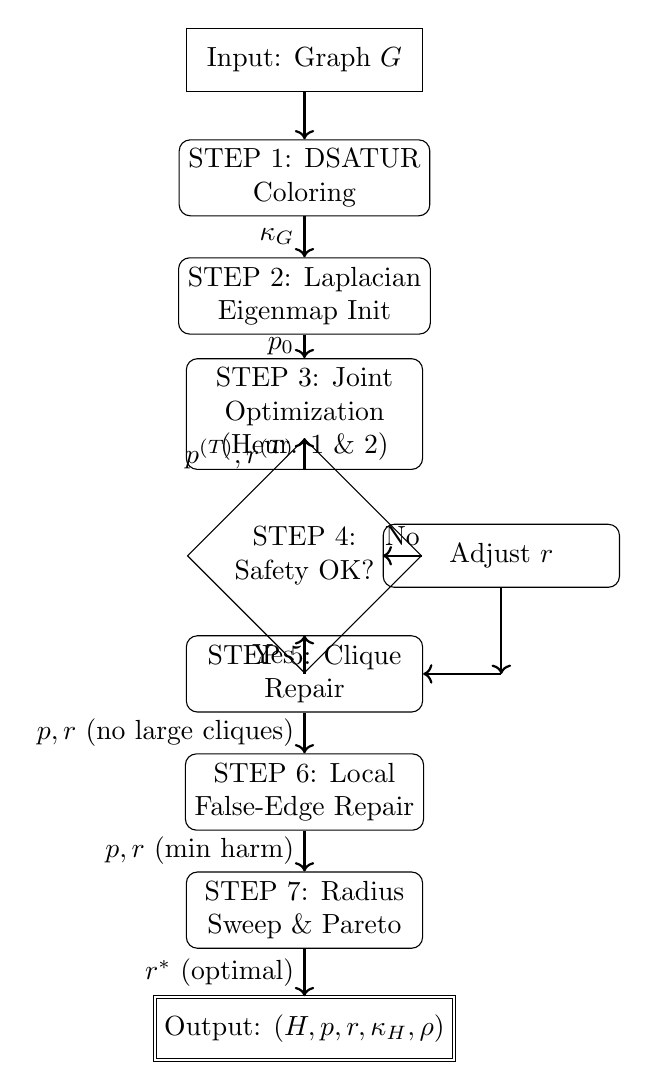
\begin{tikzpicture}[
  node distance=1.5cm,
  box/.style={rectangle, draw, minimum width=3cm, minimum height=0.8cm, align=center},
  decision/.style={diamond, draw, minimum width=2.5cm, minimum height=1cm, align=center},
  process/.style={rectangle, draw, rounded corners, minimum width=3cm, minimum height=0.8cm, align=center},
  end/.style={rectangle, draw, double, minimum width=3cm, minimum height=0.8cm, align=center}
]

% Start
\node[box] (start) at (0,0) {Input: Graph $G$};

% Step 1
\node[process] (step1) at (0,-1.5) {STEP 1: DSATUR\\Coloring};

% Step 2
\node[process] (step2) at (0,-3) {STEP 2: Laplacian\\Eigenmap Init};

% Step 3
\node[process] (step3) at (0,-4.5) {STEP 3: Joint\\Optimization\\(Heur. 1 \& 2)};

% Step 4
\node[decision] (step4) at (0,-6.3) {STEP 4:\\Safety OK?};

% Loop back if unsafe
\node[process] (step4b) at (2.5,-6.3) {Adjust $r$};

% Step 5
\node[process] (step5) at (0,-7.8) {STEP 5: Clique\\Repair};

% Step 6
\node[process] (step6) at (0,-9.3) {STEP 6: Local\\False-Edge Repair};

% Step 7
\node[process] (step7) at (0,-10.8) {STEP 7: Radius\\Sweep \& Pareto};

% Output
\node[end] (output) at (0,-12.3) {Output: $(H, p, r, \kappa_H, \rho)$};

% Edges
\draw[->,thick] (start) -- (step1);
\draw[->,thick] (step1) -- node[left] {$\kappa_G$} (step2);
\draw[->,thick] (step2) -- node[left] {$p_0$} (step3);
\draw[->,thick] (step3) -- node[left] {$p^{(T)}, r^{(T)}$} (step4);
\draw[->,thick] (step4) -- node[above] {No} (step4b);
\draw[->,thick] (step4b) -- (step4b |- step5);
\draw[->,thick] (step4b |- step5) -- (step5);
\draw[->,thick] (step4) -- node[left] {Yes} (step5);
\draw[->,thick] (step5) -- node[left] {$p, r$ (no large cliques)} (step6);
\draw[->,thick] (step6) -- node[left] {$p, r$ (min harm)} (step7);
\draw[->,thick] (step7) -- node[left] {$r^*$ (optimal)} (output);

\end{tikzpicture}
\caption{Pipeline execution flow. Each step feeds output to the next. Steps 3, 5, 6
iterate until convergence; Steps 1, 2, 4, 7 run once.}
\label{fig:pipeline}
\end{figure}

\subsection{Detailed Data Flow}

The pipeline processes data sequentially through each step:

\begin{enumerate}
  \item Input graph $G = (V, E)$ enters STEP 1 (DSATUR).
  \item DSATUR outputs coloring $\kappa_G$, which enters STEP 2 (Laplacian eigenmap).
  \item Laplacian eigenmap outputs initial placement $p_0$ and radius $r_0$, which enter STEP 3 (optimization).
  \item STEP 3 iterates 100-500 times, outputting optimized $p^{(T)}$ and $r^{(T)}$.
  \item STEP 4 safety check verifies $E(G) \subseteq E(H)$; if unsafe, $r$ is adjusted.
  \item STEP 5 clique repair detects and fixes large cliques (5-20 iterations).
  \item STEP 6 local repair removes harmful false edges (5-30 iterations).
  \item STEP 7 radius sweep evaluates 50-200 candidate radii and selects optimal $r^*$.
  \item Final step assembles certificate $(H, p, r^*, \kappa_H, \rho, |\Efalse|)$.
\end{enumerate}

\subsection{Execution Decision Logic}

The pipeline execution follows this sequence:

\begin{enumerate}
  \item \textbf{STEPS 1-2:} Always run (initialization).
  \item \textbf{STEP 3:} Run until loss converges (typically 100-500 iterations).
  \item \textbf{STEP 4:} Check safety. If unsafe, adjust $r$ and rebuild $H$.
  \item \textbf{STEP 5:} If large cliques detected, repair. Otherwise skip.
  \item \textbf{STEP 6:} If harmful false edges remain, repair. Otherwise skip.
  \item \textbf{STEP 7:} Always run (sweep and select optimal radius).
  \item \textbf{Output:} Assemble final certificate with $(H, p, r^*, \kappa_H, \rho)$.
\end{enumerate}

Each step either advances to the next step or feeds back to correct issues
(e.g., if safety fails, adjust and re-verify).

\newpage



\newpage


\section*{References}
\addcontentsline{toc}{section}{References}

\begin{thebibliography}{99}

\bibitem[Belkin \& Niyogi (2003)]{Belkin2003}
Belkin, M., \& Niyogi, P. (2003). Laplacian eigenmaps and spectral techniques for embedding and clustering. \textit{Advances in Neural Information Processing Systems}.

\bibitem[Boyd \& Vandenberghe (2004)]{Boyd2004}
Boyd, S., \& Vandenberghe, L. (2004). \textit{Convex optimization}. Cambridge University Press.

\bibitem[Brelaz (1979)]{Brelaz1979}
Brelaz, D. (1979). New methods to color the vertices of a graph. \textit{Communications of the ACM}, 22(4), 251--256.

\bibitem[Breu \& Kirkpatrick (1998)]{Breu1998}
Breu, H., \& Kirkpatrick, D. G. (1998). On the complexity of recognizing unit disk graphs. \textit{Journal of Computational Geometry and Theory of Applications}.

\bibitem[Bomze et al. (1999)]{Bomze1999}
Bomze, I. M., et al. (1999). The maximum clique problem. In \textit{Handbook of combinatorial optimization} (pp. 1--74).

\bibitem[Chung (1997)]{Chung1997}
Chung, F. R. K. (1997). \textit{Spectral graph theory} (Vol. 92). American Mathematical Society.

\bibitem[Cormen et al. (2009)]{Cormen2009}
Cormen, T. H., Leiserson, C. E., Rivest, R. L., \& Stein, C. (2009). \textit{Introduction to algorithms} (3rd ed.). MIT Press.

\bibitem[Ebadi et al. (2021)]{Ebadi2021}
Ebadi, S., et al. (2021). Quantum phases from competing short-and long-range interactions in an optical lattice. \textit{Nature}, 595, 227--232.

\bibitem[Fiedler (1973)]{Fiedler1973}
Fiedler, M. (1973). Algebraic connectivity of graphs. \textit{Czechoslovak Mathematical Journal}, 23(2), 298--305.

\bibitem[Fruchterman \& Reingold (1991)]{Fruchterman1991}
Fruchterman, T. M. J., \& Reingold, E. M. (1991). Graph drawing by force-directed placement. \textit{Software: Practice and experience}, 21(11), 1129--1164.

\bibitem[Golumbic (1980)]{Golumbic1980}
Golumbic, M. C. (1980). \textit{Algorithmic graph theory and perfect graphs}. Academic Press.

\bibitem[Graham et al. (2022)]{Graham2022}
Graham, T. M., et al. (2022). Multi-qubit entanglement and algorithms on a programmable neutral-atom quantum processor. \textit{Nature}, 604, 457--462.

\bibitem[Henriet et al. (2021)]{Henriet2021}
Henriet, L., et al. (2021). Quantum computing with neutral atoms. \textit{Quantum}, 5, 528.

\bibitem[Heppes (2003)]{Heppes2003}
Heppes, A. (2003). On the packing density of circles and spheres. \textit{Mathematika}.

\bibitem[Jungck et al. (2021)]{Jungck2021}
Jungck, D., et al. (2021). On the complexity of UDG recognition and related problems. In \textit{Computational Geometry}.

\bibitem[Kirkpatrick et al. (1983)]{Kirkpatrick1983}
Kirkpatrick, S., Gelatt, C. D., \& Vecchi, M. P. (1983). Optimization by simulated annealing. \textit{Science}, 220(4598), 671--680.

\bibitem[Lovasz (1983)]{Lovasz1983}
Lovasz, L. (1983). Kneser's conjecture, chromatic number, and homotopy. \textit{Journal of Combinatorial Theory, Series A}, 34(3), 319--324.

\bibitem[Madsen et al. (2023)]{Madsen2023}
Madsen, K. T., et al. (2023). Scalable photonic platform for quantum information. \textit{Nature}, 606, 75--81.

\bibitem[Miettinen (2014)]{Miettinen2014}
Miettinen, K. (2014). \textit{Nonlinear multiobjective optimization}. Springer.

\bibitem[Nesterov (2004)]{Nesterov2004}
Nesterov, Y. (2004). Introductory lectures on convex optimization: A basic course. \textit{Applied Optimization}, 87.

\bibitem[Preskill (2018)]{Preskill2018}
Preskill, J. (2018). Quantum computing in the NISQ era and beyond. \textit{Quantum}, 2, 79.

\bibitem[Roberts (1969)]{Roberts1969}
Roberts, F. S. (1969). Recent progresses in combinatorics. Academic Press.

\bibitem[Saffman et al. (2010)]{Saffman2010}
Saffman, M., Walker, T. G., \& Molmer, K. (2010). Quantum computing with neutral atoms. \textit{Reviews of Modern Physics}, 82(3), 2313.

\bibitem[Scholl et al. (2022)]{Scholl2022}
Scholl, P., et al. (2022). Quantum computing hardware for neutral atoms. \textit{Nature}, 605, 202--206.

\bibitem[Tutte (1954)]{Tutte1954}
Tutte, W. T. (1954). On the chromatic polynomial. \textit{Journal of Combinatorial Theory}, 2, 145--155.

\bibitem[Welsh \& Powell (1967)]{Welsh1967}
Welsh, D. J. A., \& Powell, M. B. (1967). An upper bound for the chromatic number of a graph and its application to timetabling problems. \textit{The Computer Journal}, 10(1), 85--89.

\bibitem[West (2001)]{West2001}
West, D. B. (2001). \textit{Introduction to graph theory} (2nd ed.). Prentice Hall.

\end{thebibliography}

\end{document}